
%*******************************************************
% Chapter 1
%*******************************************************

\myChapter{Markov processes}

\begin{refsection}

   An important class of stochastic processes is provided by the so-called
   Markov processes. 
   Markov processes are ubiquitous.
   They are a relevant ingredient for  
   stochastic modelling and they provide the theoretical basis of important
   statistical and coomputational techniques, ranging
from Markov-chain Montecarlo to hidden Markov models, discussed in later
parts.
   This chapter serves as an introduction to
   their definitions and first properties, and illustrates few beginning examples. The
   material is indispensable also for later chapters. 

   The following stochastic processes \emph{need not} to be Markovian.
   They can be Markovian in some special cases but they do not need to be
   Markovian in general 
   and allow for special treatment.
   For example, the simple  random walk is Markovian; the self-avoiding random
   walk is a prototypical example of a \emph{non}-Markovian process.
   For this reason, these processes will be discuss in later chapters:
   \begin{itemize}
      \item random walks;
      \item branching processes.
   \end{itemize}
   As prototypes of Markov processes we will discuss:
   \begin{itemize}
      \item Erenfest urn;
      \item \google{} \pagerank{} ranking algorithm;
      \item Applications of Markov processes to shopping;
      \item Solution of the coupon problem via Markov chains.
   \end{itemize}
   In later chapters, we will discuss modern topics like
   \begin{itemize}
      \item Markov chain Montecarlo and Metropolis-Hasting algorithm in
	 computational statistical mechanics and computational Bayesian
	 inference;
      \item Hidden Markov models.
      \end{itemize}
      Both heavily relies on Markov processes.
      The stochastic calculus and the chapter on stochastic differential
      equation makes use of Wigner integrals which are based on Markov
      processes.
	 

      \begin{figure}
	 \centering
	 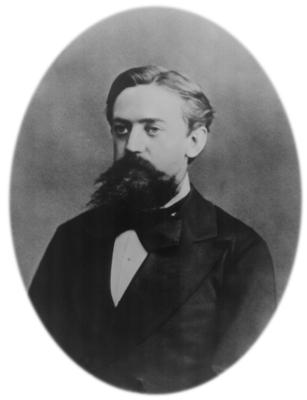
\includegraphics[width=.40\textwidth]{AAMarkov}
	 \caption{Russian mathematician Andrei Andreyevich Markov
	    (1856--1922), the father of Markov processes.}
      \end{figure}

      \section{Markov property}

      Intuitively speaking,
      Markov processes are \emph{memoryless}: the probability of evolving from
      the current state to the 
      next one does not depend on the previous history of the process.
      The exact mathematical implementation of this concept can look a bit
      technical for Markov processes defined on continuous state spaces and
      continuous index space, but for finite settings it should be easier to
      grasp.
      For this reason, we first define the general notion for arbitrary
      (continuous) processes but later we will mainly focus on the finite
      setting, where Markov processes are more often called ``Markov chains''.
      Markov chains  will be enough for most of our purposes.
      General Markov processes occur however in many situations (Brownian
      motion, Markovian evolution of open quantum systems, etc); for this
      reason, we give the general definitions.


      \section{Ergodicity}
      \section{Stationary  distribution}

      \section{Remarks on non-Markovian
	 processes}
      \footcite{Van-Kampen:1998}

      

      

      \section{The coupon problem revisited}   
      \section{Erenfest urn}
      \section{Shopping model}
      \section{\google{} \pagerank{} algorithm}
In the early days of web search engine, 


Web search engines usually work in this way:
\begin{inparaenum}[(a)]
   \item Web Crawling 
   \item Indexing 
   \item Ranking 
\end{inparaenum}
First of all, an automated Web crawler retrieves and stores information from the HTML
markup of several many web pages. 
Data is analyzed and stored in a index database for use in later queries. 
Finally, when a query is performed by the user, the list of matching results
needs to be sorted by some criteria (ranking).


The \pagerank{} algorithm was 
has a lot of interesting mathematics behind it.  
In this note we will use the \pagerank{} algorithm a  a prototypical model and
as a pathfinder to explore and to illustrate some interesting mathematics behind
it.
We will give also a toy implementation of the algorithm to start playing with
it so to discover some of its features. 



\printbibliography[heading=subbibliography]
\end{refsection}
